\documentclass{article}
\usepackage{latexsym}
\usepackage{amssymb,amsmath}
\usepackage{custom2}
\usepackage{graphicx} % for figures
\usepackage{epstopdf} % so can use EPS or PDF figures
\usepackage{caption}
\usepackage{subcaption}
\usepackage{url}
\usepackage{amssymb,amsfonts}
\usepackage[all,arc]{xy}
\usepackage{enumerate}
\usepackage{mathrsfs}
\usepackage{booktabs}
\usepackage[pdftex]{hyperref}
\usepackage{lscape}
\usepackage{xcolor}
\usepackage{natbib}

\captionsetup{justification=RaggedRight, singlelinecheck=false}
\newcommand{\ra}[1]{\renewcommand{\arraystretch}{#1}}
\newcommand{\argmax}{\text{argmax}}
\newcommand{\Tr}{\text{Tr}}
%\newtheorem{claim}{Claim}
\newtheorem{ass}{Assumption}

\addtolength{\evensidemargin}{-.5in}
\addtolength{\oddsidemargin}{-.5in}
\addtolength{\textwidth}{1.4in}
\addtolength{\textheight}{1.4in}
\addtolength{\topmargin}{-.5in}

\pagestyle{empty}

\begin{document}
\begin{center}
\Large

\end{center}


\vspace{0pt}

\begin{center}
{\bf \LARGE{Conflict and Strategy in Collective Computation}}
\end{center}

\section{Abstract}
Groups of individuals making decisions in noisy environments perform collective computations in many biological systems, ranging in size from a brain made of billions of neurons to social groups made up of tens of monkeys. In each of these systems, pairs of individuals make decisions about their relative values. We use a leaky integrator model, a set of stochastic differential equations describing how decision variables change over time, to model the decision process. The decisions made between each pair form a directed network over the whole group. The degree of consensus in the group about each individual's value, as determined by the decision network, is a collective computation that is informative about the individuals' true values. We find that differences in the model when it is applied to neural and social systems do not affect the accuracy of decisions.  We find that conflicts of interest in the decision process affect individuals with low values the most and that conflicts of interest can incentivize these individuals to make more accurate decisions. We find that when pairwise decisions are accurate, local properties of the decision network are the most informative, but when accuracy decreases global properties are more informative. Finally, we find that the shape of the distribution of consensus scores is determined by the waiting costs of those decisions. 

\section{Keywords }
collective computation, noisy learning, leaky integrator, decisions, social network, consensus, power, social structure

\section{Introduction} 
Many biological systems perform collective computation.  When presented with a set of moving dots, the brain, made up of billions of neurons, can decide whether the dots are moving left or right, even if the difference in the sizes of the groups moving either direction is not very large. A group of quorum sensing bacteria can sense its cell density and start to produce toxic, phosphorescent, or colorful molecules only when the density is sufficiently high. Flocks of birds and schools of fish can stay together and navigate with beautiful coordinated motion. In social groups of primates, the distribution of the degree of consensus about each monkey�s ability to use force is informative about the animals� abilities and the animals use estimates of this emergent property to decide how to behave. In each of these examples, the individual members of the group make decisions based on noisy environmental information and a function of or algorithm acting on those individual decisions determines the group�s output. This two-step process allows the group to produce a successful output or behavior, despite computational limitations of its members and the conflicts of interest between them. While these examples come from quite different systems, the similarity in the phenomena suggest there may be common principles underlying collective computation in all of them.

 The sequential probability ratio test (SPRT) is the optimal way to decide between two alternatives in a noisy environment in the sense that for a given amount of time the SPRT is the most accurate algorithm and for a given error rate the SPRT reaches a decision most quickly.  The algorithm works by keeping track of the amount of evidence supporting one alternative and deciding in favor of that alternative once that amount is sufficiently high or deciding against it once that amount is sufficiently low. While this algorithm assumes the decider has perfect memory, in reality this is rarely the case and a simple way to model memory loss is to assume that the amount of evidence decays back toward 0 at teach point in time. This forgetful model of decision-making can be transformed into a leaky integrator model, a set of stochastic differential equations (SDEs) describing how the variables accumulating evidence for each alternative change over time. The random walk described by the SDEs is biased by the true state of the environment. This model is applicable to any system in which an individual with imperfect memory gathers evidence and chooses the alternative for which he has gathered more support.  The leaky integrator model, while a powerful for modeling noisy learning dynamics, has been applied rather phenomenologically, and we seek here to justify its use with a mechanistic derivation.

In this paper, we will study a group of individuals, each pair of which is trying to make a decision about their relative values. Each individual will have a decision variable indicating how much evidence it has accumulated and a threshold.  If the decision variable reaches the threshold, the individual will signal that a decision has been made. Both individuals involved in the decision value making a correct and fast decision. Since it takes time to gather enough evidence to make a correct decision, there is a tradeoff between accuracy and speed. Additionally, each individual might prefer that the decision be made in their favor, whether or not they truly have a higher value.  This introduces a conflict of interest. The thresholds are the strategies they use to negotiate accuracy, speed, and their personal preferences.

The leaky integrator model has been applied to neural decision-making, and it successfully explains and predict performance in a number of experiments  \citep{Eckhoff:2008uq, Brown:2005fk,Feng:2009kl,Bogacz:2006uq}. In this application, each of two neural populations responds to evidence for either left or right motion.  The SDEs describe how the firing rates of the two populations change over time and a decision is made once one the difference in firing rates is sufficiently high. Usually, the visual stimulus driving this decision process is a set of dots, some percentage of which are moving coherently either left or right and the rest of which are moving randomly.  The bias in the SDEs is in favor of the direction in which the coherent dots are moving.  However, this process could be used by neural populations deciding between any two possibilities, for example between up and down motion or between two colors, and a group of neural populations could be used to distinguish between or rank a whole set of possibilities. 

While the SPRT has been applied to animal conflicts  \citep{Froment:2010fk}, to our knowledge the leaky integrator model has not been. In this application, each of two animals has a belief about its dominance with respect to the other which increases or decreases as the animal wins or loses fights against its opponent. The SDEs describe how these beliefs change over time. The source of evidence is the fight history between the two animals. Even if one animal is stronger and tends to win fights, the outcome of a fight is affected by the identity and presence of each animal's allies, motivation levels,  external environmental variables, and other stochastic factors, which introduce noise.   The bias in the SDEs is in favor of the animal that is more likely to win. Once an animals' opinion goes below a threshold, it decides to agree to be subordinate to the other. A correct decision is one in which the weaker individual makes this agreement.  In pigtailed macaques ({\it Macaca nemestrina}) and other species of macaques, there is a formal subordination signal that an animal can use to communicate its agreement to the subordinate role in their relationship \citep{Flack:2007kx, Flack:2006fk,Flack:2004oq, Waal:1985fk,Caldecott:1986uk,Preuschoft:2004ly}.  This signal marks the end of the decision process.

The leaky integrator model can thus be used to describe a decision being made between each pair of individuals in a group.  These decisions form a directed network, each edge of which reflects a decision about the relative values of the nodes it connects. In many systems, the degree of consensus in a group about each individuals' state is informative about the individuals'  true states and affects the individuals' functional behavior \cite{Brush:2013fk}. In previous work, we developed a number of network metrics to measure the degree of consensus in the group about each node and we found a few that produced scores that were predictive of individuals' functional behaviors \cite{Brush:2013fk,Flack:2006uq}. The output of one of these consensus measures being applied to a decision network would be a set of consensus scores, a collective computation which would be informative about the individuals' true states.

In the social case, this consensus is referred to as social power. In macaques, power is a useful variable since it reflects the animals' true abilities and the animals themselves do use estimates of their peers' and their own power to decide how to behave \cite{Flack:2004oq,Flack:2006fk,Flack:2006uq}.  The distribution of power scores in an empirical group of pigtailed macaques is heavy tailed and this allows the individuals in the tail to perform different functions in the social group than the rest of its members \cite{Flack:2005uq,Flack:2006fk,Flack:2006uq}.  Further, the shape of the power distribution varies across species of macaques \cite{Caldecott:1986uk,Flack:2004oq,Preuschoft:2004ly,Waal:1985fk,Thierry:2000ij}, and it is an open question whether this variation can be explained by differences in the underlying distributions of fighting abilities, by differences in the way animals in different species resolve their differences, or through other mechanisms. This kind of consensus may be important in neural systems, as well.  A number of neural populations may respond to or encode different environmental stimuli or variables.  The consensus in a group of neural populations about the value of a number of environmental stimuli could help the brain make decisions about the relative values of many possibilities. 

There are thus three factors affecting the collective computation: the statistical properties of the environment, the strategies individuals use to make decisions about their relative values, and the method of measuring consensus from a network of decisions.  In this paper, first we derive the leaky integrator model from a simple mechanistic description of the accumulation of information, making two simplifying assumptions about the timescales on which probabilistic events occur \cite{Gillespie:2000fk}. We then use this model to answer the following questions. Do differences in the decision making model as it is applied to neural and social systems affect the accuracy of the decision process? What threshold strategies should individuals with conflicting interests use to make decisions in a group context? How do the individuals� threshold strategies affect the collective computation? What function of the decision network produces the most informative collective computation? How well does our model describe empirical social systems?

\section{Model} 
\subsection{Stochastic differential equations }    
%% make debt to Gillespie clearer

There are two possible types of environmental evidence: in the neural system, a dot can move either left or right and in the social system, a fight can be won by one animal or another.  For clarity in the following we will refer to these left or right dots, but the biological interpretation of the two types of inputs depends on the system. There are two decision variables, $X_1$ and $X_2$. In the absence of any input, the decision variables leak back towards $0$ with rate $\ell$.  (A table of all variables used in the text is given in Table \ref{variables}.)  If there is no input, then over a period length $\tau$ a decision variable decreases as $X(t+\tau)=(1-\ell\tau)X(t)$.

Each decision variable responds positively to one type of input and negatively to the other.  In the neural case, one neural population responds positively to left dots and negatively to right dots and the other neural population does the opposite.  In the social case, one animal's estimate of its own dominance increases when it wins fights and decreases when it loses fights, and the other animal's estimate does the opposite. Neither decision variable has perfect memory.  Specifically, $X_1$ increases by a boost $b$ when it sees a left dot and decrements by $-b$ when it sees a right dot, and conversely for $X_2$.     
To calculate the variables at time $t+\tau$, we  count how many times each of type of input occurred in the time since $t$ and add the changes resulting from these events to the background leaky estimate (as in \cite{Gillespie:2000fk}):
\begin{align*}
X_1(t+\tau)&=(1-\ell\tau)X_1(t)+b\times\# \text{ of left dots in }[t,t+\tau)-b\times\# \text{ of right dots in }[t,t+\tau)
\\ X_2(t+\tau)&=(1-\ell\tau)X_2(t)-b\times\# \text{ of left dots in }[t,t+\tau)+b\times\# \text{ of right dots in }[t,t+\tau). 
\end{align*}

Our first assumption is that the rates at which the two types of inputs occur is constant over time.  We can thus describe the number of each type of event with a Poisson random variable, $N_\text{L}$ and $N_\text{R}$.  We rewrite our basic equations to give 
\begin{align*}
X_1(t+\tau)&=(1-\ell\tau)X_1(t)+bN_\text{L}-bN_\text{R}
\\ X_1(t+\tau)&=(1-\ell\tau)X_2(t)-bN_\text{L}+bN_\text{R}.
\end{align*}
If events happen at a rate $r$ and the event is a left dot with probability $c$ and a right dot with probability $1-c$, then the expectation of $N_L$ and $N_R$ in a period of length $\tau$ are, respectively, $\tau r c$ and $\tau r(1-c)$. In the neural case, $c$ is related to the ``coherence'' of the visual stimulus.  A $c$ close to $0$ or $1$ means that most of the events are of one type or the other and the decision is easier to make than when $c$ is close to $.5$.

If enough events happen in the period of time from $t$ to $t+\tau$ then we can approximate the Poisson random variables with Normal random variables with mean and variance equal to the mean of the Poisson random variables.  Our second assumption, then, is that the period of time of length $\tau$ is long enough to make this approximation. Let $Z_\text{L}$ and $Z_\text{R}$, be independent standard Normal random variables, i.e. with mean $0$ and standard deviation $1$.  Then our equations for $X_i(t+\tau)$ become
\begin{align*}
X_1(t+\tau)&=(1-\ell\tau)X_1(t)+b\bigg(\tau rc+\sqrt{\tau rc}Z_{\text{L}}\bigg)-b\bigg(\tau r(1-c)+\sqrt{\tau r(1-c)}Z_{\text{R}}\bigg)
\\X_2(t+\tau)&=(1-\ell\tau)X_2(t)-b\bigg(\tau rc+\sqrt{\tau rc}Z_{\text{L}}\bigg)+b\bigg(\tau r(1-c)+\sqrt{\tau r(1-c)}Z_{\text{R}}\bigg).
\end{align*}
Finally, as we make the period of time shorter and shorter, making $\tau$ infinitesimally small, these equations become stochastic differential equations,
\begin{equation}
\begin{array}{ll}
dX_1&=\bigg(-\ell X_1(t)+br(2c-1)\bigg)dt+\bigg(b\sqrt{rc}\bigg)dW_\text{L}t-\bigg(b\sqrt{r(1-c)}\bigg)dW_\text{R}t
\\dX_2&=\bigg(-\ell X_2(t)-br(2c-1)\bigg)dt-\bigg(b\sqrt{rc}\bigg)dW_\text{L}t+\bigg(b\sqrt{r(1-c)}\bigg)dW_\text{R}t
\end{array}
\end{equation}
where $dW_{\text{L}}$ and $dW_{\text{R}}$ are independent Brownian motions representing, respectively, the left and right inputs.  The assumptions about the timescales on which inputs occur are particularly reasonable in the social system, although the successful application of this type of model to neural populations implies they are not unreasonable in that system.  In Table \ref{variables}, we list the inputs, outputs, and variables of the decision model and how they should be interpreted in the neural and social systems.


\subsection{Reaching a decision }
Each decision variable, $X_1$ and $X_2$, accumulates information about the stimulus.  The sign and size of the two variables indicate how much evidence there is for each possible decision outcome.  When a lot of evidence for the first possibility has been observed, $X_1$ will be large and positive, and similarly for the second possibility.  If the difference in the variables can be observed, the difference indicates the relative strengths of the evidence for either possibility. If $Y=X_1-X_2$, when $Y$ is large enough the system decides on $X_1$ and when $Y$ is low enough the system decides on $X_2$.  Specifically, there are two thresholds, $T_2$ and $T_1$ such that if $Y>T_1$ the decision is for $X_1$ and if $Y<-T_2$ the decision is for $X_2$.  However, it may be the case that the difference in the variables cannot be observed.  In this case, the decision depends on whether $X_1$ or $X_2$ hits a threshold first.  Again, there are two thresholds, $T_2$ and $T_1$, and if $X_1<-T_1$ the decision is for $X_1$ and if the $X_2<-T_2$ the decision is for $X_2$. 

In the neural system, the two stochastic equations describing the activity of the two neural populations integrating environmental evidence are often reduced to the one-dimensional equation describing the difference in the activity levels to make the system easier to analyze \cite{Brown:2005fk,Bogacz:2006uq,Feng:2009kl}.  However, in the social system we are considering, we cannot make any assumptions about the existence of a third party evaluating the difference in the opinions of the two animals.  A ``decision," i.e. the emission of a signal from one of the two animals, is only reached when one of the two animals' opinions goes below a certain threshold.  The social system is therefore inherently two-dimensional, whereas the neural system may be adequately described by one dimension.  In Table \ref{differences}, we compare how the decision is made and how the decision process is optimized in the two systems.

\subsection{Utility of the decision }
The thresholds affect how long the decision takes and the probabilities with which each output is decided upon.  A good decision is one that reaches the correct output quickly, i.e. the expected time until a decision is reached (decision time, DT) and the probability that an incorrect decision is made (error rate, ER) are low.   However, it is impossible to minimize both simultaneously since waiting longer and accumulating more evidence makes the decision more accurate and conversely.  It may also be the case that each individual prefers one output over the other, regardless of which is ``correct''.  In the social case, an animal would prefer that its partner agreed to be subordinate, whether or not it is truly stronger.  In the neural case, different neural populations may receive different rewards if the decision reaches different outputs, regardless of which of the alternatives is ``true."  In these cases, a variable wants to maximize the probability that his preference is reached (probability of preference being chosen, $\text{PP}_i$).    

To describe the tradeoffs between error rate, decision time, and preference, we quantify the utility of the decision process by introducing three weights, $w_1$, $w_2$, and $w_3$ such that $w_1+w_2+w_3=1$.  These weights describe how the three quantities are prioritized.  For individual $i$, we define
\begin{equation*}
U_{i}=w_1\text{ER}+w_2\text{DT}+w_3(1-\text{PP}_i).
\end{equation*}
The decision is better if $U_i$ is lower.  In the social system, $w_2$ can be interpreted as the cost of fighting since when $w_2$ is higher, the time spent fighting until a decision is reached is more costly.  Similarly, $w_3$ can be interpreted as the benefit from being the dominant animal in a pair. In both cases, $w_3$ represents how stubborn the individuals are about their preferences. If $w_3\gneq 0$ and the individuals prefer different outcomes, neither can simultaneously be satisfied since $\text{PP}_1=1-\text{PP}_2$.

As show in the Appendix, each of the three decision properties, ER, DT, and PP satisfies a partial differential equation that depends on the SDEs and the parameters of the model. There are analytical solutions to these equations when the system of SDEs is reduced to one dimension. However, we were not able to find an analytical solution for the full two-dimensional system and we therefore used numerical methods to solve the PDEs in this case.

\subsection{Optimal thresholds }
An individual-- either a neural population or a monkey-- can be engaged in either a single decision or in many decisions at once.  In the social system, for example, an animal wants to decide whether it is dominant or subordinate to every other member of its social group.  For any pair of individuals, each has a utility, $U_1$ and $U_2$, and consequently each has a Nash equilibrium threshold such that, if they choose those thresholds, neither has an incentive to choose another.  Similarly, in a group of individuals, each individual $i$ has a utility $U_{ij}$ from its decision process with individual $j$.  His total utility is given by the average of these, $\langle U_{ij}\rangle _j$. These lead to an optimized set of thresholds such that no individual has an incentive to choose another threshold.

Since an individual is trying to use the same algorithm to learn about every one else, he is constrained to have only one decision threshold for each of these decision processes.  In order to consistently assign the difficulties with which all pairs in a group make decisions, we assign each individual a value $a_i$ and the difficulty with which the pair $i,j$ makes a decision increases with the difference in abilities, i.e. $c_{ij}$ is an increasing function of $|a_i-a_j|$. In the social system, these values can be interpreted as the fighting abilities of the animals.The optimal decision threshold in this group context depends on the distribution of difficulties ($c_{ij}$) of the decision an individual will have to make and the thresholds of the other individuals.    

 We use the following procedure to find optimal thresholds as a function of position in the group.  We repeatedly draw a set of fighting abilities from a uniform distribution; we find the optimal thresholds for each set, and then find the average optimal threshold as a function of an animal's order in the set of fighting abilities. To find the optimal thresholds for a given set of fighting abilities, we turn the difference in fighting abilities between each pair into the difficulty of the decision they have to make ($c$).  For an initial set of thresholds, we find $U_{ij}$ for each animal $i$ in each of its decisions and then average $\langle U_{ij}\rangle_j$ across all the animals with which it is engaged in a decision process.  We then allow each animal to choose a threshold that optimizes $\langle U_{ij}\rangle_j$ with respect to the rest of the group's thresholds and we iterate these choices until no animal chooses a new threshold.  

\subsection{Collective computation }
We are interested in how the consensus about the value of each individual emerges out of the decision process.  (In the social system, an animal's social power depends on the consensus in the group about its fighting ability \cite{Brush:2013fk,Flack:2004oq,Flack:2006uq}.)  Given an interaction network, there are many ways to measure the consensus present in the group about each individual's value \cite{Brush:2013fk, Flack:2006uq}. These formalisms assign a consensus score to each node in the network (interpreted as a power score in the social system).  In the following we consider four  consensus formalisms.  The first and simplest is simply the number of nodes sending decisions to each animal (number of signalers).  The second is the number of decisions received by each node, which is a finer measure than the first.  The third is the entropy of the distribution of the number of decisions sent to each individual, which measures gives a coarse measurement of how uniformly all other animals in the group behave with respect to a focal individual.  The fourth is the eigenvector centrality of the signaling network, which measures how central each node is in the global structure of the network.  For more details see \cite{Brush:2013fk}. 

To use these measures, we need to construct an interaction network between individuals in the group.  For each random set of fighting abilities, we let the animals optimize their thresholds, which give the probability that each pair will reach either decision and the expected time it will take.  We use these probabilities to generate a set of decisions between all pairs.  We use the convention that a decision is sent from $i$ to $j$ if in their decision $j$'s preference prevailed.  (In the social system, $i$ sends a subordination signal to $j$ to communicate his agreement to be subordinate.) To incorporate the time it takes for a decision to be reached and allow for multiple decisions to be sent, we say that $i$ sends $j$ a number of decisions equal to $1$ minus the expected decision time.  At each point in time $t$, the weight of the edge from $i$ to $j$ is $0$ if the expected decision time is greater than $t$ (i.e. a decision has not been made) and is given by the number of signals sent from $i$ to $j$ otherwise. Using many random sets of fighting abilities, for each consensus formalism and each point in time $t$, we can find the mutual information between the consensus scores from the network at $t$ and the true values. We can also find the average skewness of the set of consensus scores.

\section{Results}
\subsection{Decision making is as accurate without a third party arbiter. }
First we compare the decision making process in the full two-dimensional system and in a reduced one-dimensional system to see whether decisions are made more accurately or quickly in one or the other.  To make the systems directly comparable, we assume in both cases that the thresholds are symmetric, i.e. $T_1=T_2$.  We find that the two-dimensional decision is as accurate as the one-dimensional decision.  That is, for a given expected time to reach a decision, the two-dimensional decision will reach the correct decision with the same probability. Because they perform equally well and because the two-dimensional system is more appropriate for the social system (and perhaps the neural system as well), we use the two-dimensional system in the rest of our analyses. While the results come from an analysis of the two-dimensional system, they should also apply to the reduced system.
%Accuracy decreases as leak rates ($\ell$) become higher, but increases when the strength of the input ($c$) is higher.

\subsection{A conflict of interests incentivizes individuals in the bottom of the group to make more accurate decisions. }
The Nash equilibrium thresholds for a pair of individuals depend on whether the individuals are minimizing error rate, maximizing probability of their preference, or minimizing decision time.  If accuracy of the decision is the only thing that matters ($w_1=1$), the weaker individual will set his threshold as low as possible and the stronger animal will set his threshold as high as possible since if the decision is correct the weaker animal gives up first. When personal preference matters ($w_3>0)$ and there is a conflict of interest between the individuals, both will set their threshold high since there is no incentive for the individuals to stop accumulating evidence. As the importance of decision time increases (i.e. waiting costs increase), both individuals will lower their thresholds in order to reach the decision more quickly, whatever that decision may be (Figure \ref{nasheq}).  Notice that decision time and personal preference lead both animals to have the same thresholds whereas the individuals have different thresholds when accuracy is important. The accuracy with which a pair using Nash thresholds can reach a decision is highest when only error rate matters ($w_1=1$) and decreases as either decision time or personal preference become important (Figure \ref{nasheq}).  

In a group, an individual's position in the group affects how it makes the tradeoff between error rate, preference and decision time.  As in a pair, prioritizing accuracy tends to lead animal's at the top of the group to set high thresholds and those at the bottom to set low thresholds. Prioritizing personal preferences, on the other hand, tends to lead all individuals to set high thresholds (Figure \ref{groupeq}). The difference in an individual's threshold between when accuracy is important and when personal preferences are important is largest for the individuals at the bottom of the group. Individuals towards the top will set high thresholds in either case. Individuals toward the bottom, however, will set lower thresholds when they prioritize accuracy then when they prioritize personal preferences. This is because choosing a higher threshold would increase waiting time in decisions with respect to all individuals and decrease the accuracy of its decisions with respect to higher animals, and it would only slightly increase the accuracy of its decisions with respect to other low individuals. In other words, individuals at the bottom of the group sacrifice some accuracy in their decisions with respect to each other in order to decrease their overall decision times. 

This leads to the slightly counterintuitive result that making personal preferences less important (i.e. having a larger conflict of interest) and making accuracy more important actually decreases the average accuracy of the decisions made between individuals at the bottom of the group. This in turn leads to a very slight increase in the average accuracy of all pairs in the group (Figure \ref{groupeq}).  For every measure of consensus, the mutual information between the consensus scores and the true values increases with average pairwise accuracy.  Thus, the information content of the consensus scores is also slightly higher when the individuals prioritize personal preference rather than error rate.

\subsection{Global network structure provides the most information when accuracy is high but imperfect and when the network is developing. }
First, we consider the mutual information between the consensus formalisms applied to a fully formed decision network and the true values. It is interesting to note that for each of the four types of formalisms we consider, there are regions of the simplex given by the optimization weights that make that the most informative formalism. When pairwise decisions are on average quite accurate, the number of decisions received is the most informative about the underlying values (Figure \ref{bestmetric}).  This makes sense since when each edge in the decision network accurately reflects the difference in value between individuals, the number of edges received is informative about an individual's position in the group.  When the pairwise decisions are less accurate, global structure of the decision network provides information about values that the individual relationships do not, so eigenvector centrality is the measure that is the most informative about values.  

The differences in mutual information given by each formalism are very small, but the clear pattern that the best formalism depends on waiting costs needs explanation. The number of signalers consistently overestimates individuals' value.  When accuracy is fairly high, this bias makes it uninformative about value.  However, when accuracy is quite low, this consistent bias actually make the number of signalers more informative than measures whose errors are less predictable. When accuracy is lower still, none of the measures are very informative, but entropy correctly gives the lowest individuals low scores, giving it an edge over the other measures.

When the number of signals or number of signalers out-perform the other formalisms, the differences in performance are very small. When eigenvector centrality is the best, on the other hand, it clearly outperforms the others (Figure \ref{bestmetric}). Eigenvector centrality is consistently the most informative formalism on a network that is not fully formed (Figure \ref{bestmetric}). 

\subsection{The skewness of the power distribution is maximized when decisions are moderately accurate. }
For each measure of consensus in the decision network, we find the average skewness of the distribution of consensus scores of a group using optimal thresholds, as they depend on optimization weight.  We find that for all measures skewness is maximized at intermediate waiting costs and does not depend strongly on the tradeoff between error rate and preference (Figure \ref{skewness}). (Results for number of signalers are shown in Figure \ref{skewness} and others are similar).  When waiting costs are low and accuracy is high, the decisions accurately represent the individuals' true  abilities so the distribution of number of signalers accurately represents the distribution of abilities, which is not very right-skewed.  When waiting costs are high and accuracy is low, all individuals receive decisions from a similar number of others, giving a distribution that is quite uniform and not right-skewed.  At intermediate waiting costs, the decisions sent to individuals with low to middle abilities are very noisy so that the individuals in the bottom and middle of the group receive signals from similar numbers of individuals.  However, all individuals make accurately decisions with the top few individuals, giving them high scores, resulting in a right-skewed distribution.


\subsection{Decisions in a group take longest between individuals with similarly high abilities. }
Difficult decisions tend to (but do not always) take longer than easier decisions.  In a social system, the difficult of a decision increases as a pair becomes more similar.  In a group of decision makers, the absolute value of two individuals, as well as the difference in their values, affects how quickly they can make a decision.  When waiting costs are low, the pairs that take the longest to reach a decision are those with similar fighting abilities, but pairs with different abilities also take a fairly long time.  When waiting costs are high, all pairs reach decisions quickly.  At intermediate costs, most pairs can reach a decision quite quickly, except those who have similar and high abilities (Figure \ref{groupeq}).  Pairs with similar and high abilities always take as long or longer to make a decision than any other pairs do.
 

\section{Discussion}

We derive a pair of stochastic differential equations that describe how two individuals accumulate evidence from a noisy environment.  The model can be equally well applied to the firing rates of neural populations observing a visual stimulus and the beliefs of two monkeys about their relative dominance based on their fighting history.   We first compare the simplified version of the model that is frequently used to describe the neural system and the full version we need to describe the social system.  We then consider a population of individuals using this model to make decisions to investigate the best way of making a collective computation, how to improve the accuracy of this computation and how the shape of the power structure in the social system depends on the accuracy of decisions.  Finally, we find a model output that is comparable to empirical observations.

Either the absolute value of the decision variables or the difference in their values can determine the outcome of the decision.  We find that, for a given decision time, the accuracy of the decision does not depend on which of these mechanisms is used.  In order for the difference in variables to be used, a third party arbiter needs to be present to evaluate the value of each decision variable and find their difference.  In the brain, it might be the case that there is a third neural population whose activity depends on the two populations gathering external evidence, but in a social group, there is not a third party informing how a pair of animals should establish their subordination-dominance relationship.  The fact, then, that the model does not depend on the existence of this third party arbiter means that it can be equally well applied whether or not it is present.

The decisions between pairs of individuals give rise to a network of decisions between all members of a group. A group of individuals will have some degree of consensus about the status of each individual. This consensus is the result of a collective computation that depends on individual behaviors.  There are many different ways of measuring this consensus and each represents a different way of performing the collective computation \cite{Brush:2013fk,Flack:2006uq}. When the accuracy of pairwise decisions is relatively high but imperfect, then a global metric like eigenvector centrality is the most informative about the true states of the nodes. When pairwise accuracy is quite low, then a coarse measure like the number of signalers or the entropy of decisions received outperforms a finer measure like the number of decisions received.

As network scientists, if we are presented with an interaction network, we would like to know how to measure the consensus present in the network about each node.  If we have a sense of the accuracy with which the edges reflect true differences in the states of the nodes, this result gives a rule of thumb for how to pick a measure of consensus. However, since eigenvector centrality always performs optimally or close to optimally on a fully formed network and it performs optimally on a network that is still forming, eigenvector centrality would would generally be a good choice. 

As members of a social group about which they would like to have information, the monkeys may use these measures (or approximations of them) to estimate their own and their peers' abilities. In previous work, we found that both eigenvector centrality and measures of the number of decisions received produced scores that were informative about animals' functional behavior in a group of pigtailed macaques.  This may be informative about the optimization weights the animals in that group are using.  If so, it would suggest that decision time is less important than a combination of error rate and the probability of being dominant. If animals in different species do prioritize fighting costs and the benefits from being dominant (i.e. decision time and probability of preference)  differently, we might expect to find that those animals use different properties of their social networks to estimate the power structure of the group.  

Individuals in biological systems are likely to be selfish and stubborn, both in order to maximize their own welfare and because prioritizing accuracy requires knowing which the ``right'' answer is.  The accuracy of the collective computation depends on how the individuals make the tradeoff between personal preference and accuracy, regardless of which measure is used to make the computation.  We expected to find that individuals valuing their preference at the expense of the correct output would tend to make decisions that were less accurate.  In a pair, this holds true.  However, when there is a group of individuals all making this tradeoff, valuing preferences over accuracy improves the accuracy with which individuals in the bottom of the group resolve their differences, increasing the average accuracy of the whole group. This overall accuracy translates into a more accurate collective computation.   

Usually only two neural populations are included in models of neural decision making (although see XXX).  Further, it is usually assumed that neural populations in the brain value accuracy, since the whole organism receives a benefit from making a correct decision in a short time.  But it is possible that different neural populations receive different rewards from making different decisions, regardless of which decision is the ``correct'' one.  Only by considering a group of decision makers do we find the surprising result that the accuracy of a collective computation can be improved by introducing conflicting interests.  This might suggest that in situations where a group of neural populations are recruited to make a decision, we could expect to find that they have different preferences, rather than all valuing accuracy. Our result also has interesting implications for designing networks whose properties we would like to use to make computations.

The skewness of the power structure that results from this collective computation in social groups of macaques has important functional consequences \cite{Flack:2004oq,Flack:2006fk}. We find that for most measures of power the skewness of the distribution of power scores is maximized at intermediate waiting costs.  In our data, we observe a right-skewed distribution of power \cite{Brush:2013fk,Flack:2006uq}.  To the extent that our model recapitulates the empirical system, this would suggest that waiting costs are neither the only priority nor are they ignored completely.

Different species of macaque have stereotypical power structures with different amounts of skewness \cite{Flack:2004oq,Preuschoft:2004ly,Waal:1985fk}.  One explanation might be that the distribution of fighting abilities is different from species to species, for instance if there is more or less variation in body size.  However, our model suggests that even if the underlying distribution of fighting abilities are identical, the priorities given to preference, error rate, and waiting costs can affect the distribution of power.  The benefit of having a partner agree to be subordinate, the benefit of reaching the ``correct" agreement, and the costs of fighting may vary from species to species, causing variation in the shape of the power structure.

Individual-based models and computer simulations have previous been used to explain the social structures of macaques \cite{Hemelrijk:2011fk,Hausfater:1981fk}. In a more complicated model, the ``aggressiveness'' of animals moving in a spatially explicit area affected the shape of the dominance hierarchy \cite{Hemelrijk:2011fk}.  While the mechanisms of that model are quite different, ``aggressiveness'' could be argued to be similar to disregarding fighting costs and prioritizing preference.  Neither the authors of that work nor we found that a difference in the underlying distribution of fighting abilities is required to change the distribution of dominance or power.  In other words, in both models, the collective computation that results in a power structure depends more on how the individuals interact and collect information than on the distribution of fighting abilities. 

It is difficult to assess whether decisions in empirical systems are being made accurately, but it is easier to measure how long they take.  In a group, each pair of individuals experiences the difference in their abilities, but their absolute positions within the group also matter.  In data from a captive population of macaques, we observe that pairs of animals with high abilities reach agreements about their relative dominance but that pairs of animals with low abilities sometimes do not reach such agreements (JC Flack, unpublished data).  In our model, decisions between pairs who have similar and high abilities always  take as long or longer than decisions between any other pairs.  This discrepancy indicates that our simple model is missing a level of social complexity that could explain this empirical pattern.  

There are (at least) two modifications to the model that we expect would produce results closer to the empirical observations.  First, in the model, the rates at which animals fight each other do not depend on the abilities of the animals.  However, it is likely that animals with lower abilities are less mobile and encounter their peers at a lower rate than animals with higher abilities who are more free to range throughout the group.  In the model, this heterogeneity in encounter rate would make the decisions between animals with low encounter rates take longer.  Second, in the model, all animals value preference, error rate, and waiting costs equally.  However, it is likely that the benefits from receiving a subordination signal from a partner and the costs of fighting depend on both animals' abilities.  If animals with low ability  do not value an agreement with other animals with similar abilities, there would be less incentive for them to reach an agreement.  These types of heterogeneity would make our model more biologically realistic when applied to the social system, but without them it is general enough to be applied to a number of systems in which collective computations are being performed.  

We consider two systems, a neural and a social, and our model reduces to previously studied ``war of attrition'' games in the game theory literature when the abilities of the two individuals are equal.  The similarities between these three frameworks-- neural decision making, social decision making, and game theory-- suggest that there are common principles of decision making through conflict that are applicable to a number of systems. Conflict and strategy are not usually ascribed to the neural model, and the war of attrition is not usually thought of as a process through which the pair of competitors reaches a decision about an external truth.  Our work is a first step toward unifying these different frameworks and better understanding the importance of conflict and strategy in collective computation.
%%other applications?

\begin{figure}[ht]
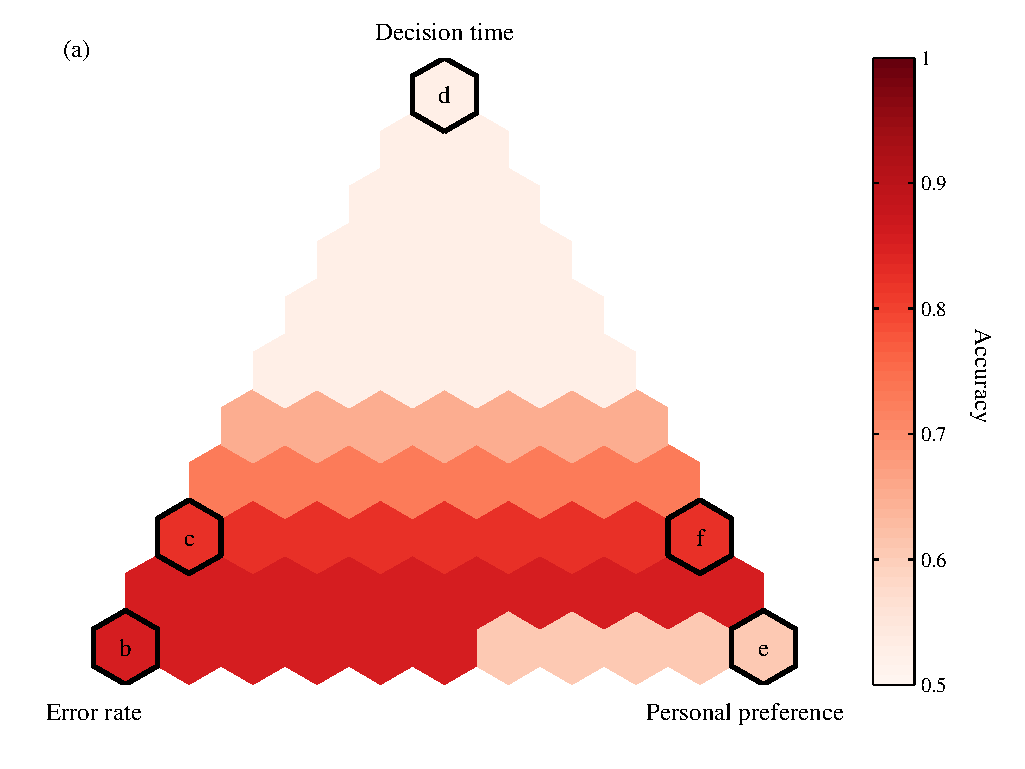
\includegraphics[]{pairwiseaccuracy.pdf}
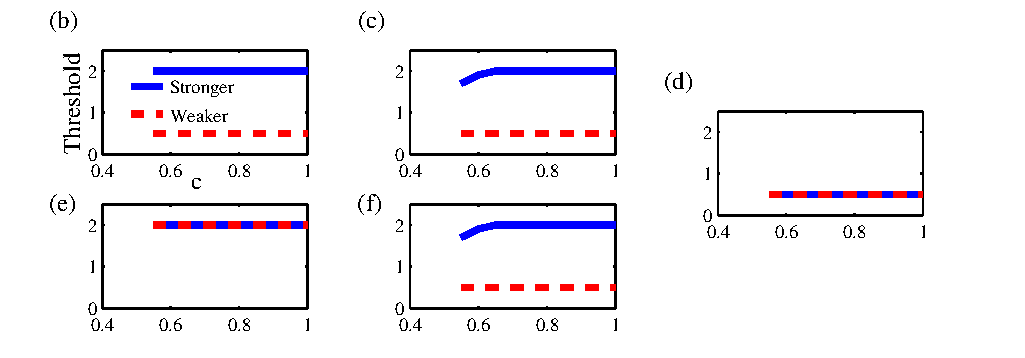
\includegraphics[]{nasheq_thresholds.pdf}
\caption{\label{nasheq} The accuracy of a pair using Nash equilibrium thresholds decreases as the weight given to decision time increases.  (a) In the upper panel, the color indicates the accuracy of a decision made by a pair making a difficult decision ($c=.55$) using Nash equilibrium thresholds, as a function of the optimization weights, $w_1$, $w_2$, $w_3$.  In the lower left corner of the simplex, only error rate matters ($w_1=1$).  In the upper corner, only decision time matters ($w_2=1$).  In the lower right corner, only preference matters ($w_3=1$). Accuracy decreases as $w_2$ increases but is not greatly affected by a tradeoff between $w_1$ and $w_3$. In (b)-(g) we show how the Nash equilibrium thresholds depend on the difficulty of the decision ($c$). The optimization weights for each panel are indicated in the simplex with the corresponding letter.  }
\end{figure}

\begin{figure}[ht]
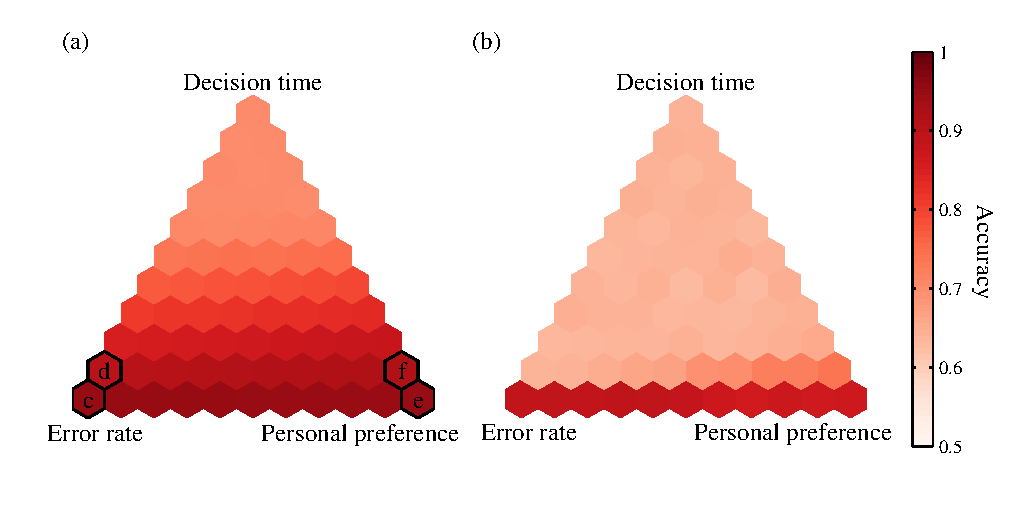
\includegraphics[width=\textwidth]{groupaccuracy.pdf}
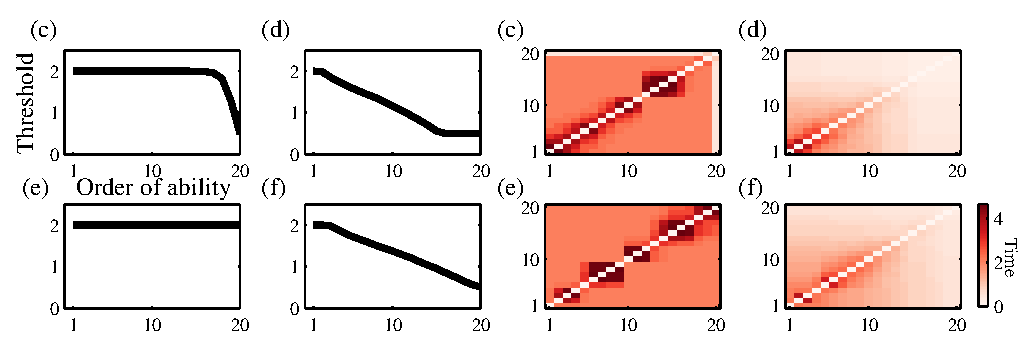
\includegraphics[width=\textwidth]{groupeq_thresholds.pdf}
\caption{\label{groupeq}   The accuracy of a group using optimal thresholds decreases as the weight given to decision time increases.  In the upper panels, the color indicates (a) the average accuracy of the whole group and (b) the average accuracy of the decisions between individuals in the bottom quartile using optimal thresholds, as a function of the optimization weights, $w_1$, $w_2$, $w_3$.  In the lower left corner of the simplex, only error rate matters ($w_1=1$).  In the upper corner, only decision time matters ($w_2=1$).  In the lower right corner, only preference matters ($w_3=1$). Both bottom-quartile and total accuracy decrease as $w_2$ increases, and the increase in bottom-quartile accuracy as $w_3$ increases drives a slight increase in total accuracy.  In (c)-(f) we show how the group-context optimal thresholds (left panels) and decision time for each pair (right panels) depends on the true order of value where $1$ is the strongest individual and $20$ is the weakest. The optimization weights for each panel are indicated in the simplex with the corresponding letter.  For low waiting costs (c and e), it takes longest for pairs with similar values to reach a decision.  For slightly higher waiting costs (d and f), it takes longer for pairs with similar and high values to reach a decision.}

\end{figure}

\section{Figures}
\begin{figure}[ht]
%\begin{minipage}{.66\linewidth}
%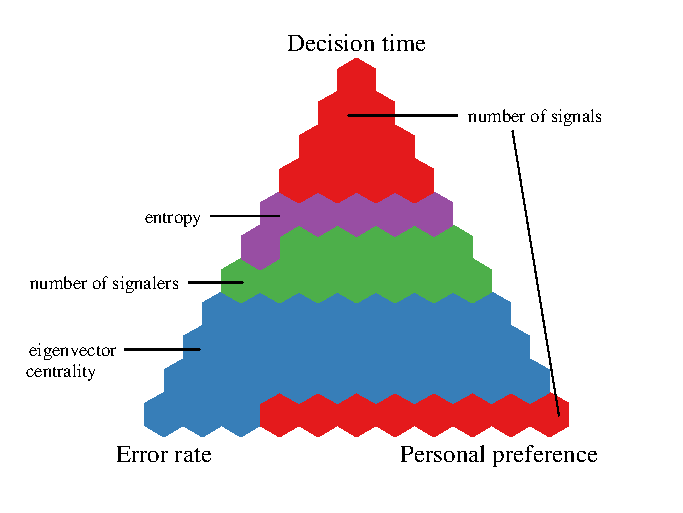
\includegraphics[width=\linewidth]{mostinformative.pdf}
%\end{minipage}
%\begin{minipage}{.44\linewidth}
%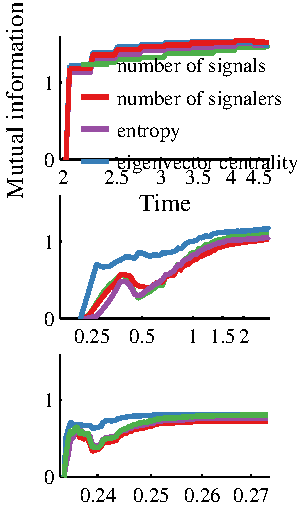
\includegraphics[width=.66\linewidth]{infogrowth.pdf}
%\end{minipage}
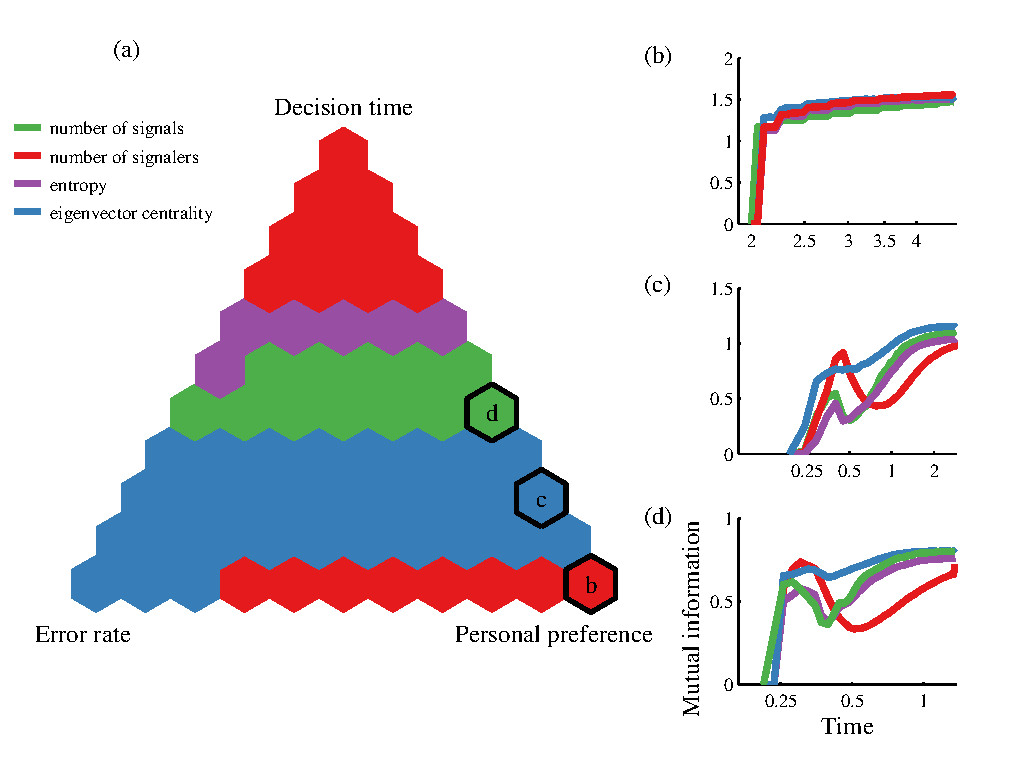
\includegraphics[width=\textwidth]{info.pdf}
\caption{\label{bestmetric} The best method to use for measuring consensus in the decision network depends on how accurate decisions are on average.  (a) In the left panel, the color indicates the most informative consensus formalisms. In the lower left corner of the simplex, only error rate matters ($w_1=1$).  In the upper corner, only decision time matters ($w_2=1$).  In the lower right corner, only preference matters ($w_3=1$). In (b)-(d) we show how the mutual information of each consensus formalisms increases over time. The optimization weights for each panels are indicated in the simplex with the corresponding letter.}
\end{figure}


\begin{figure}[ht]
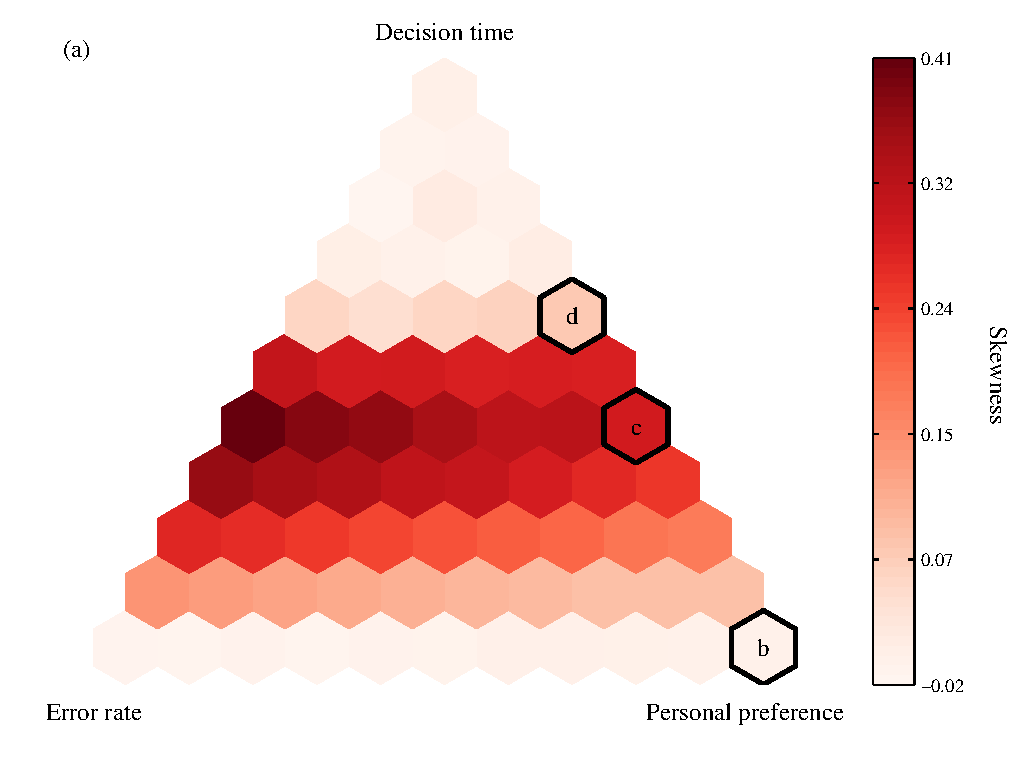
\includegraphics[width=\textwidth]{skewness.pdf}
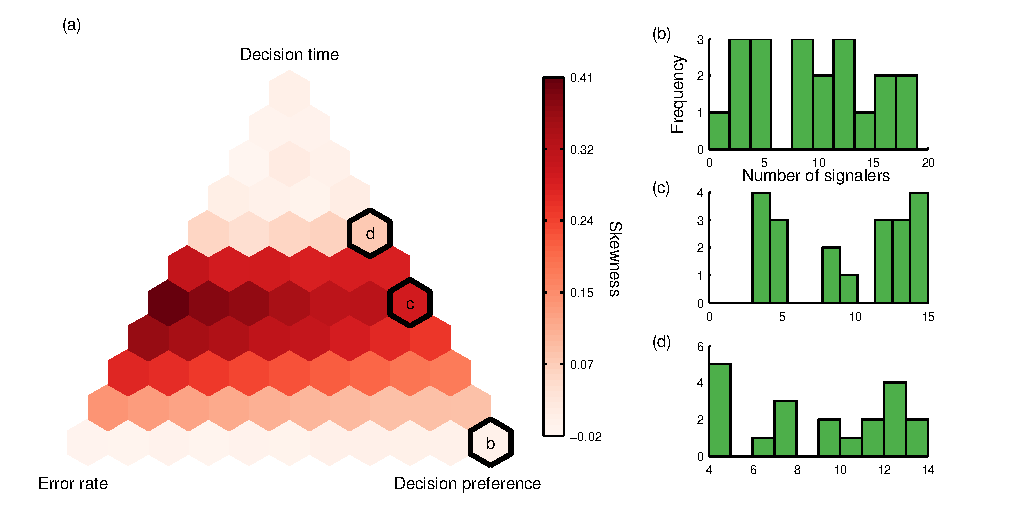
\includegraphics[width=\textwidth]{skewness_histograms.pdf}
\caption{\label{skewness} The average skewness of the distribution of the number of signalers is maximized at intermediate waiting costs. In the upper panel, the color indicates the average skewness of the distribution of a group using optimal thresholds, as a function of the optimization weights, $w_1$, $w_2$, $w_3$. In the lower left corner of the simplex, only error rate matters ($w_1=1$).  In the upper corner, only decision time matters ($w_2=1$).  In the lower right corner, only preference matters ($w_3=1$). In (b)-(d) we show a histogram for a representative distribution of the number of signalers for a group using the optimization weights as indicated in the simplex with the corresponding letter.}
\end{figure}

\begin{table}[ht]
\centering
\caption{\label{variables}{\bf  Collective computations.} }
\ra{1.3}
\begin{tabular}{@{}lllll@{}}
System & Environmental information & Individual &   Individual decision & Collective computation \\
\cmidrule{1-5} 
brain & dots moving left or right & neural population & to stop firing & brain-level decision for left or right
\\  social group & fights won or lost & monkey & to emit a subordination signal & power structure
\\  quorum sensing & signaling molecule & bacteria & to produce signaling molecule & toxicity or phosphorescence
\\ flock movement & environment & bird & where to fly and how quickly & flock movement and navigation
\end{tabular}
\end{table}


\begin{table}[ht]
\centering
\caption{\label{variables}{\bf  Variables and interpretations in neural and social systems.} }
\ra{1.3}
\begin{tabular}{@{}lllll@{}}
Variable & Interpretation & Neural &   Social \\
\cmidrule{1-4} 
& input & dots moving left or right & fights won or lost
\\$c$ & strength of input & coherence of dots & prob. of stronger animal winning
\\$X_1,X_2$ & decision variables &  firing rates of neural populations & opinions about relative dominance
\\ $w_1$ & error rate weight & reward from being ``right" & reward from being ``right"
\\ $w_2$ & decision time weight & penalty for taking a long time & costs of fighting
\\ $w_3$ & prob. of preference weight & ? & benefit from receiving signal
\\ & decision & subject indicates left or right & one animal emits subordination signal
\\ & correct decision & subject chooses correct direction & weaker animal signals
\end{tabular}
\end{table}

\begin{table}[ht]
\centering
\caption{\label{differences}{\bf  Comparison of model in its original application to neural systems, in an extended application to neural systems, and its application to social systems.} Differences are highlighted in red.}
\ra{1.3}
\begin{tabular}{@{}lllll@{}}
&Original neural & & Social \\
\cmidrule{2-3} \cmidrule{4-4} 
dimensionality & $1$  && $2$
\\decision & difference hits a threshold  && \fcolorbox{red}{white}{one var. hits a threshold}
\\ optimality criterion &  reward from being ``right" && reward from being ``right"
\\ & decision time && decision time
\\ & && \fcolorbox{red}{white}{reward from  receiving signal}
\\optimization depends on & input strength && input strength
\\ & noise && noise
\\ & leak rate && leak rate
\\ & && \fcolorbox{red}{white}{other animal's threshold}
\end{tabular}
\end{table}

\pagebreak
\section{Appendix}

\subsection{Derivation of PDEs for waiting time and accuracy \label{pdes_deriv}}

\pagebreak
\nocite{*}
\bibliographystyle{plain}
\bibliography{signaling_model}

\end{document}


